\chapter{Formal Proof}
\label{chapter:ref}

\section{Formulate Statement}

\subsection{ Redefinition of Narrow RevTerminate Principle}
Compared to informal logic proofs, our formal logic proof requires stricter definitions. 
Here is the Narrow RevTerminate Principle:
``Given a reversible abstract machine with a finite number of total states, it will inevitably terminate from any initial state.''

First of all, we define the initial state.  Given a state, if it is not the next state of any other state, we call it an initial state.

\begin{code}%
\>[2]\AgdaFunction{is-initial} %
\AgdaSymbol{:} %
\AgdaField{State} %
\AgdaSymbol{→} %
\AgdaPrimitive{Set} %
\AgdaSymbol{\AgdaUnderscore{}}\<%
\\
%
\>[2]\AgdaFunction{is-initial} %
\AgdaBound{st} %
\AgdaSymbol{=} %
\AgdaFunction{∄[} %
\AgdaBound{st'} %
\AgdaFunction{]} %
\AgdaSymbol{(}\AgdaBound{st'} %
\AgdaOperator{\AgdaField{↦}} %
\AgdaBound{st}\AgdaSymbol{)}\<%
\\
\>[0]\<%
\end{code}

Secondly, we define the terminate of a reversible machine.
Starting from the initial state $st_{0}$, we use $st_{0}$ $\mapsto$* $st_{n}$ to indicate that $st_{0}$ can reach $st_{n}$ by traversing a finite number of steps.

\begin{code}%
    \>[2]\AgdaKeyword{data} %
    \AgdaOperator{\AgdaDatatype{\AgdaUnderscore{}↦*\AgdaUnderscore{}}} %
    \AgdaSymbol{:} %
    \AgdaField{State} %
    \AgdaSymbol{→} %
    \AgdaField{State} %
    \AgdaSymbol{→} %
    \AgdaPrimitive{Set} %
    \AgdaSymbol{(}\AgdaPrimitive{L.suc} %
    \AgdaBound{ℓ}\AgdaSymbol{)} %
    \AgdaKeyword{where}\<%
    \\
    \>[2][@{}l@{\AgdaIndent{0}}]%
    \>[4]\AgdaInductiveConstructor{◾} %
    \AgdaSymbol{:} %
    \AgdaSymbol{\{}\AgdaBound{st} %
    \AgdaSymbol{:} %
    \AgdaField{State}\AgdaSymbol{\}} %
    \AgdaSymbol{→} %
    \AgdaBound{st} %
    \AgdaOperator{\AgdaDatatype{↦*}} %
    \AgdaBound{st}\<%
    \\
    %
    \>[4]\AgdaOperator{\AgdaInductiveConstructor{\AgdaUnderscore{}∷\AgdaUnderscore{}}} %
    \AgdaSymbol{:} %
    \AgdaSymbol{\{}\AgdaBound{st₁} %
    \AgdaBound{st₂} %
    \AgdaBound{st₃} %
    \AgdaSymbol{:} %
    \AgdaField{State}\AgdaSymbol{\}} %
    \AgdaSymbol{→} %
    \AgdaBound{st₁} %
    \AgdaOperator{\AgdaField{↦}} %
    \AgdaBound{st₂} %
    \AgdaSymbol{→} %
    \AgdaBound{st₂} %
    \AgdaOperator{\AgdaDatatype{↦*}} %
    \AgdaBound{st₃} %
    \AgdaSymbol{→} %
    \AgdaBound{st₁} %
    \AgdaOperator{\AgdaDatatype{↦*}} %
    \AgdaBound{st₃}\<%
    \\
    \>[0]\<%
\end{code}

If a state $st_{0}$ have no next state, we call it a stuck state.

\begin{code}%
\>[2]\AgdaFunction{is-stuck} %
\AgdaSymbol{:} %
\AgdaField{State} %
\AgdaSymbol{→} %
\AgdaPrimitive{Set} %
\AgdaSymbol{\AgdaUnderscore{}}\<%
\\
%
\>[2]\AgdaFunction{is-stuck} %
\AgdaBound{st} %
\AgdaSymbol{=} %
\AgdaFunction{∄[} %
\AgdaBound{st'} %
\AgdaFunction{]} %
\AgdaSymbol{(}\AgdaBound{st} %
\AgdaOperator{\AgdaField{↦}} %
\AgdaBound{st'}\AgdaSymbol{)}\<%
\\
\>[0]\<%
\end{code}

The termination of a reversible machine means that given an initial state, it will reach a stuck state.

\begin{code}%
\>[2]\AgdaFunction{is-stuck} %
\AgdaSymbol{:} %
\AgdaField{State} %
\AgdaSymbol{→} %
\AgdaPrimitive{Set} %
\AgdaSymbol{\AgdaUnderscore{}}\<%
\\
%
\>[2]\AgdaFunction{is-stuck} %
\AgdaBound{st} %
\AgdaSymbol{=} %
\AgdaFunction{∄[} %
\AgdaBound{st'} %
\AgdaFunction{]} %
\AgdaSymbol{(}\AgdaBound{st} %
\AgdaOperator{\AgdaField{↦}} %
\AgdaBound{st'}\AgdaSymbol{)}\<%
\\
\>[0]\<%
\end{code}

Finally, we define ``a reversible abstract machine with a finite number of total states.''
Here is the definition of Fin in agda.  A Fin $\mathbb{N}$ set have exactly $\mathbb{N}$ elements.

\begin{code}%
\>[2]\AgdaFunction{is-stuck} %
\AgdaSymbol{:} %
\AgdaField{State} %
\AgdaSymbol{→} %
\AgdaPrimitive{Set} %
\AgdaSymbol{\AgdaUnderscore{}}\<%
\\
%
\>[2]\AgdaFunction{is-stuck} %
\AgdaBound{st} %
\AgdaSymbol{=} %
\AgdaFunction{∄[} %
\AgdaBound{st'} %
\AgdaFunction{]} %
\AgdaSymbol{(}\AgdaBound{st} %
\AgdaOperator{\AgdaField{↦}} %
\AgdaBound{st'}\AgdaSymbol{)}\<%
\\
\>[0]\<%
\end{code}

We construct a bijection between the set of states and Fin $\mathbb{N}$.
It is as if all states are indexed by an element in the Fin $\mathbb{N}$ set.

\begin{code}%
\>[2]\AgdaFunction{is-stuck} %
\AgdaSymbol{:} %
\AgdaField{State} %
\AgdaSymbol{→} %
\AgdaPrimitive{Set} %
\AgdaSymbol{\AgdaUnderscore{}}\<%
\\
%
\>[2]\AgdaFunction{is-stuck} %
\AgdaBound{st} %
\AgdaSymbol{=} %
\AgdaFunction{∄[} %
\AgdaBound{st'} %
\AgdaFunction{]} %
\AgdaSymbol{(}\AgdaBound{st} %
\AgdaOperator{\AgdaField{↦}} %
\AgdaBound{st'}\AgdaSymbol{)}\<%
\\
\>[0]\<%
\end{code}

Combining the definition above, we have the exact definition of Narrow RevTerminate Principle:


\begin{code}%
    \>[2]\AgdaFunction{Finite-State-Termination} %
    \AgdaSymbol{:} %
    \AgdaSymbol{∀} %
    \AgdaSymbol{\{}\AgdaBound{N} %
    \AgdaBound{st₀}\AgdaSymbol{\}}\<%
    \\
    \>[2][@{}l@{\AgdaIndent{0}}]%
    \>[4]\AgdaSymbol{→} %
    \AgdaField{State} %
    \AgdaOperator{\AgdaFunction{⤖}} %
    \AgdaDatatype{Fin} %
    \AgdaBound{N}\<%
    \\
    %
    \>[4]\AgdaSymbol{→} %
    \AgdaSymbol{(}\AgdaBound{has-next} %
    \AgdaSymbol{:} %
    \AgdaSymbol{∀} %
    \AgdaSymbol{(}\AgdaBound{st} %
    \AgdaSymbol{:} %
    \AgdaField{State}\AgdaSymbol{)} %
    \AgdaSymbol{→} %
    \AgdaRecord{Dec} %
    \AgdaSymbol{(}\AgdaFunction{∃[} %
    \AgdaBound{st'} %
    \AgdaFunction{]} %
    \AgdaSymbol{(}\AgdaBound{st} %
    \AgdaOperator{\AgdaField{↦}} %
    \AgdaBound{st'}\AgdaSymbol{)))}\<%
    \\
    %
    \>[4]\AgdaSymbol{→} %
    \AgdaFunction{is-initial} %
    \AgdaBound{st₀}\<%
    \\
    %
    \>[4]\AgdaSymbol{→} %
    \AgdaFunction{∃[} %
    \AgdaBound{stₙ} %
    \AgdaFunction{]} %
    \AgdaSymbol{(}\AgdaBound{st₀} %
    \AgdaOperator{\AgdaDatatype{↦*}} %
    \AgdaBound{stₙ} %
    \AgdaOperator{\AgdaFunction{×}} %
    \AgdaFunction{is-stuck} %
    \AgdaBound{stₙ}\AgdaSymbol{)}\<%
    \\
    \>[0]\<%
\end{code}

\subsection{ Redefinition of Broad RevTerminate Principle }
Here is the Broad RevTerminate Principle:
``Given a reversible abstract machine, it will inevitably terminate from any initial state with a finite number of reachable states.''

Most of the definitions are the same as those in the Narrow RevTerminate Principle:

For a state to be initial, no other state should have it as their next state.

\begin{code}%
\>[2]\AgdaFunction{is-initial} %
\AgdaSymbol{:} %
\AgdaField{State} %
\AgdaSymbol{→} %
\AgdaPrimitive{Set} %
\AgdaSymbol{\AgdaUnderscore{}}\<%
\\
%
\>[2]\AgdaFunction{is-initial} %
\AgdaBound{st} %
\AgdaSymbol{=} %
\AgdaFunction{∄[} %
\AgdaBound{st'} %
\AgdaFunction{]} %
\AgdaSymbol{(}\AgdaBound{st'} %
\AgdaOperator{\AgdaField{↦}} %
\AgdaBound{st}\AgdaSymbol{)}\<%
\\
\>[0]\<%
\end{code}

$st_{0}$ $\mapsto$* $st_{n}$ indicates that $st_{0}$ can reach $st_{n}$ by traversing a finite number of steps.

\begin{code}%
    \>[2]\AgdaKeyword{data} %
    \AgdaOperator{\AgdaDatatype{\AgdaUnderscore{}↦*\AgdaUnderscore{}}} %
    \AgdaSymbol{:} %
    \AgdaField{State} %
    \AgdaSymbol{→} %
    \AgdaField{State} %
    \AgdaSymbol{→} %
    \AgdaPrimitive{Set} %
    \AgdaSymbol{(}\AgdaPrimitive{L.suc} %
    \AgdaBound{ℓ}\AgdaSymbol{)} %
    \AgdaKeyword{where}\<%
    \\
    \>[2][@{}l@{\AgdaIndent{0}}]%
    \>[4]\AgdaInductiveConstructor{◾} %
    \AgdaSymbol{:} %
    \AgdaSymbol{\{}\AgdaBound{st} %
    \AgdaSymbol{:} %
    \AgdaField{State}\AgdaSymbol{\}} %
    \AgdaSymbol{→} %
    \AgdaBound{st} %
    \AgdaOperator{\AgdaDatatype{↦*}} %
    \AgdaBound{st}\<%
    \\
    %
    \>[4]\AgdaOperator{\AgdaInductiveConstructor{\AgdaUnderscore{}∷\AgdaUnderscore{}}} %
    \AgdaSymbol{:} %
    \AgdaSymbol{\{}\AgdaBound{st₁} %
    \AgdaBound{st₂} %
    \AgdaBound{st₃} %
    \AgdaSymbol{:} %
    \AgdaField{State}\AgdaSymbol{\}} %
    \AgdaSymbol{→} %
    \AgdaBound{st₁} %
    \AgdaOperator{\AgdaField{↦}} %
    \AgdaBound{st₂} %
    \AgdaSymbol{→} %
    \AgdaBound{st₂} %
    \AgdaOperator{\AgdaDatatype{↦*}} %
    \AgdaBound{st₃} %
    \AgdaSymbol{→} %
    \AgdaBound{st₁} %
    \AgdaOperator{\AgdaDatatype{↦*}} %
    \AgdaBound{st₃}\<%
    \\
    \>[0]\<%
\end{code}

If a state have no next state, we call it a stuck state.

\begin{code}%
\>[2]\AgdaFunction{is-stuck} %
\AgdaSymbol{:} %
\AgdaField{State} %
\AgdaSymbol{→} %
\AgdaPrimitive{Set} %
\AgdaSymbol{\AgdaUnderscore{}}\<%
\\
%
\>[2]\AgdaFunction{is-stuck} %
\AgdaBound{st} %
\AgdaSymbol{=} %
\AgdaFunction{∄[} %
\AgdaBound{st'} %
\AgdaFunction{]} %
\AgdaSymbol{(}\AgdaBound{st} %
\AgdaOperator{\AgdaField{↦}} %
\AgdaBound{st'}\AgdaSymbol{)}\<%
\\
\>[0]\<%
\end{code}

Before defining ``a finite number of reachable states'', we need to define the ``set of reachable states.''
$st_{0}$ $\mapsto$[m] $st_{m}$ means $st_{0}$ reaches $st_{m}$ exactly after m steps.
For all the m and corresponding $st_{m}$ that satisfy $st_{0}$ $\mapsto$[m] $st_{m}$, this is called ``set of reachable states.''

\begin{code}%
    \AgdaFunction{∃[} %
    \AgdaBound{m} %
    \AgdaFunction{]} %
    \AgdaFunction{∃[} %
    \AgdaBound{stₘ} %
    \AgdaFunction{]} %
    \AgdaSymbol{(}\AgdaBound{st₀} %
    \AgdaOperator{\AgdaDatatype{↦[}} %
    \AgdaBound{m} %
    \AgdaOperator{\AgdaDatatype{]}} %
    \AgdaBound{stₘ}\AgdaSymbol{)} %
    \\
    \>[0]\<%
\end{code}

In Agda, each element of reachable states set is represented as a tuple. 

\vspace{1em}

\usetikzlibrary{graphs, positioning, quotes, shapes.geometric}

\begin{document}
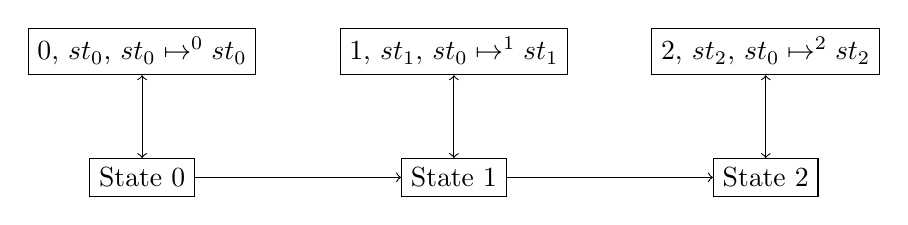
\begin{tikzpicture}[node distance=10pt]
    \node[draw] (Description 0)  {0, $st_{0}$, $st_{0}\mapsto^{0}st_{0}$};
    \node[draw, right=30pt of Description 0] (Description 1)  {1, $st_{1}$, $st_{0}\mapsto^{1}st_{1}$};
    \node[draw, right=30pt of Description 1] (Description 2)  {2, $st_{2}$, $st_{0}\mapsto^{2}st_{2}$};
    
    \node[draw, below=30pt of Description 0]    (State 0)  {State 0};
    \node[draw, below=30pt of Description 1]    (State 1)  {State 1};
    \node[draw, below=30pt of Description 2]    (State 2)  {State 2};
    

    \graph{
        (State 0) -> (State 1) -> (State 2);
        (State 0) <-> (Description 0);
        (State 1) <-> (Description 1);
        (State 2) <-> (Description 2);
    };
\end{tikzpicture}

Then, we construct a bijection between the set of reachable states and Fin $\mathbb{N}$.

\begin{code}%
    \AgdaBound{St-Fin} %
    \AgdaSymbol{:} %
    \AgdaFunction{∃[} %
    \AgdaBound{m} %
    \AgdaFunction{]} %
    \AgdaFunction{∃[} %
    \AgdaBound{stₘ} %
    \AgdaFunction{]} %
    \AgdaSymbol{(}\AgdaBound{st₀} %
    \AgdaOperator{\AgdaDatatype{↦[}} %
    \AgdaBound{m} %
    \AgdaOperator{\AgdaDatatype{]}} %
    \AgdaBound{stₘ}\AgdaSymbol{)} %
    \AgdaOperator{\AgdaFunction{⤖}} %
    \AgdaDatatype{Fin} %
    \AgdaBound{N}\<%
    \\
\end{code}

Combining the definition above, we have the exact definition of the Broad RevTerminate Principle:

\begin{code}%
    \>[2]\AgdaFunction{Finite-Reachable-State-Termination} %
    \AgdaSymbol{:} %
    \AgdaSymbol{∀} %
    \AgdaSymbol{\{}\AgdaBound{N} %
    \AgdaBound{st₀}\AgdaSymbol{\}}\<%
    \\
    \>[2][@{}l@{\AgdaIndent{0}}]%
    \>[4]\AgdaSymbol{→} %
    \AgdaSymbol{(}\AgdaBound{St-Fin} %
    \AgdaSymbol{:} %
    \AgdaFunction{∃[} %
    \AgdaBound{m} %
    \AgdaFunction{]} %
    \AgdaFunction{∃[} %
    \AgdaBound{stₘ} %
    \AgdaFunction{]} %
    \AgdaSymbol{(}\AgdaBound{st₀} %
    \AgdaOperator{\AgdaDatatype{↦[}} %
    \AgdaBound{m} %
    \AgdaOperator{\AgdaDatatype{]}} %
    \AgdaBound{stₘ}\AgdaSymbol{)} %
    \AgdaOperator{\AgdaFunction{⤖}} %
    \AgdaDatatype{Fin} %
    \AgdaBound{N}\AgdaSymbol{)}\<%
    \\
    %
    \>[4]\AgdaSymbol{→} %
    \AgdaSymbol{(}\AgdaBound{has-next} %
    \AgdaSymbol{:} %
    \AgdaSymbol{∀} %
    \AgdaSymbol{(}\AgdaBound{st} %
    \AgdaSymbol{:} %
    \AgdaField{State}\AgdaSymbol{)} %
    \AgdaSymbol{→} %
    \AgdaRecord{Dec} %
    \AgdaSymbol{(}\AgdaFunction{∃[} %
    \AgdaBound{st'} %
    \AgdaFunction{]} %
    \AgdaSymbol{(}\AgdaBound{st} %
    \AgdaOperator{\AgdaField{↦}} %
    \AgdaBound{st'}\AgdaSymbol{)))}\<%
    \\
    %
    \>[4]\AgdaSymbol{→} %
    \AgdaFunction{is-initial} %
    \AgdaBound{st₀}\<%
    \\
    %
    \>[4]\AgdaSymbol{→} %
    \AgdaFunction{∃[} %
    \AgdaBound{stₙ} %
    \AgdaFunction{]} %
    \AgdaSymbol{(}\AgdaBound{st₀} %
    \AgdaOperator{\AgdaDatatype{↦*}} %
    \AgdaBound{stₙ} %
    \AgdaOperator{\AgdaFunction{×}} %
    \AgdaFunction{is-stuck} %
    \AgdaBound{stₙ}\AgdaSymbol{)}\<%
    \\
\end{code}

\section{Formal Logic Proof for the Narrow RevTerminate Principle}

\subsection{ Steps }

\begin{code}%
    \>[2]\AgdaFunction{Finite-State-Termination} %
    \AgdaSymbol{:} %
    \AgdaSymbol{∀} %
    \AgdaSymbol{\{}\AgdaBound{N} %
    \AgdaBound{st₀}\AgdaSymbol{\}}\<%
    \\
    \>[2][@{}l@{\AgdaIndent{0}}]%
    \>[4]\AgdaSymbol{→} %
    \AgdaField{State} %
    \AgdaOperator{\AgdaFunction{⤖}} %
    \AgdaDatatype{Fin} %
    \AgdaBound{N}\<%
    \\
    %
    \>[4]\AgdaSymbol{→} %
    \AgdaSymbol{(}\AgdaBound{has-next} %
    \AgdaSymbol{:} %
    \AgdaSymbol{∀} %
    \AgdaSymbol{(}\AgdaBound{st} %
    \AgdaSymbol{:} %
    \AgdaField{State}\AgdaSymbol{)} %
    \AgdaSymbol{→} %
    \AgdaRecord{Dec} %
    \AgdaSymbol{(}\AgdaFunction{∃[} %
    \AgdaBound{st'} %
    \AgdaFunction{]} %
    \AgdaSymbol{(}\AgdaBound{st} %
    \AgdaOperator{\AgdaField{↦}} %
    \AgdaBound{st'}\AgdaSymbol{)))}\<%
    \\
    %
    \>[4]\AgdaSymbol{→} %
    \AgdaFunction{is-initial} %
    \AgdaBound{st₀}\<%
    \\
    %
    \>[4]\AgdaSymbol{→} %
    \AgdaFunction{∃[} %
    \AgdaBound{stₙ} %
    \AgdaFunction{]} %
    \AgdaSymbol{(}\AgdaBound{st₀} %
    \AgdaOperator{\AgdaDatatype{↦*}} %
    \AgdaBound{stₙ} %
    \AgdaOperator{\AgdaFunction{×}} %
    \AgdaFunction{is-stuck} %
    \AgdaBound{stₙ}\AgdaSymbol{)}\<%
    \\
    \>[0]\<%
\end{code}

Similar to the informal logic proof, we prove the principle using the following steps:
\begin{enumerate}[1.]
    \item Starting from the initial state, continue steping into the next state.
    \item If the next state doesn't exist, then the machine terminates.
    \item Upon taking $\mathbb{N}$ steps, demonstrate a contradiction using Piegonhole Principle and No-Repeat Principle.
    \item At this point, we have proven the case within $\mathbb{N}$ steps and shown that it's impossible for the case to extend beyond $\mathbb{N}$ steps.
\end{enumerate}

\subsection{ Countdown Rule }
To realize the step of continuing to the next step, we add a step m and the corresponding state $st_{m}$.

\begin{code}%
\>[2]\AgdaFunction{is-initial} %
\AgdaSymbol{:} %
\AgdaField{State} %
\AgdaSymbol{→} %
\AgdaPrimitive{Set} %
\AgdaSymbol{\AgdaUnderscore{}}\<%
\\
%
\>[2]\AgdaFunction{is-initial} %
\AgdaBound{st} %
\AgdaSymbol{=} %
\AgdaFunction{∄[} %
\AgdaBound{st'} %
\AgdaFunction{]} %
\AgdaSymbol{(}\AgdaBound{st'} %
\AgdaOperator{\AgdaField{↦}} %
\AgdaBound{st}\AgdaSymbol{)}\<%
\\
\>[0]\<%
\end{code}

When m is less than $\mathbb{N}$, we try stepping into the next state.  
If there isn't a next state, we have reached the target stuck state.  
Otherwise, we make a recursion with the case of m increasing.
Until m equals $\mathbb{N}$, we have to prove that the case is impossible.

\begin{code}%
\>[2]\AgdaFunction{is-initial} %
\AgdaSymbol{:} %
\AgdaField{State} %
\AgdaSymbol{→} %
\AgdaPrimitive{Set} %
\AgdaSymbol{\AgdaUnderscore{}}\<%
\\
%
\>[2]\AgdaFunction{is-initial} %
\AgdaBound{st} %
\AgdaSymbol{=} %
\AgdaFunction{∄[} %
\AgdaBound{st'} %
\AgdaFunction{]} %
\AgdaSymbol{(}\AgdaBound{st'} %
\AgdaOperator{\AgdaField{↦}} %
\AgdaBound{st}\AgdaSymbol{)}\<%
\\
\>[0]\<%
\end{code}

For the method above, Agda will give a ``Termination checking failed'' error.
To make the proof terminate, we have to create a variable ``countdown'' in the statement.  
The ``countdown'' should keep decreasing until it equals to zero.  And we prove the case zero at last.
The ``countdown'' is precisely the counterpart to m.  
We keep ensuring ``cd + m $\equiv$ N.''  
In this way, the proof will terminate exactly when m equals to $\mathbb{N}$, as originally intended.

Here is the new principle with a countdown

\begin{code}%
    \>[4]\AgdaPostulate{Finite-State-Termination-With-Countdown} %
    \AgdaSymbol{:} %
    \AgdaSymbol{∀} %
    \AgdaSymbol{\{}\AgdaBound{N} %
    \AgdaBound{st₀}\AgdaSymbol{\}}\<%
    \\
    \>[4][@{}l@{\AgdaIndent{0}}]%
    \>[6]\AgdaSymbol{→} %
    \AgdaField{State} %
    \AgdaOperator{\AgdaFunction{⤖}} %
    \AgdaDatatype{Fin} %
    \AgdaBound{N}\<%
    \\
    %
    \>[6]\AgdaSymbol{→} %
    \AgdaFunction{is-initial} %
    \AgdaBound{st₀}\<%
    \\
    %
    \>[6]\AgdaSymbol{→} %
    \AgdaSymbol{∀} %
    \AgdaBound{cd} %
    \AgdaBound{m} %
    \AgdaBound{stₘ} %
    \AgdaSymbol{→} %
    \AgdaBound{cd} %
    \AgdaOperator{\AgdaPrimitive{+}} %
    \AgdaBound{m} %
    \AgdaOperator{\AgdaDatatype{≡}} %
    \AgdaBound{N} %
    \AgdaSymbol{→} %
    \AgdaBound{st₀} %
    \AgdaOperator{\AgdaDatatype{↦[}} %
    \AgdaBound{m} %
    \AgdaOperator{\AgdaDatatype{]}} %
    \AgdaBound{stₘ}\<%
    \\
    %
    \>[6]\AgdaSymbol{→} %
    \AgdaFunction{∃[} %
    \AgdaBound{stₙ} %
    \AgdaFunction{]} %
    \AgdaSymbol{(}\AgdaBound{st₀} %
    \AgdaOperator{\AgdaDatatype{↦*}} %
    \AgdaBound{stₙ} %
    \AgdaOperator{\AgdaFunction{×}} %
    \AgdaFunction{is-stuck} %
    \AgdaBound{stₙ}\AgdaSymbol{)}\<%
    \\
    \>[0]\<%
\end{code}

\subsection{ Case at N }
Here is the statement of Narrow RevTerminate Principle after n steps; we have to prove this case is impossible:

\begin{code}%
    \\
    %
    \>[4]\AgdaPostulate{Finite-State-Termination-At-N} %
    \AgdaSymbol{:} %
    \AgdaSymbol{∀} %
    \AgdaSymbol{\{}\AgdaBound{N} %
    \AgdaBound{st₀}\AgdaSymbol{\}}\<%
    \\
    \>[4][@{}l@{\AgdaIndent{0}}]%
    \>[8]\AgdaSymbol{→} %
    \AgdaField{State} %
    \AgdaOperator{\AgdaFunction{⤖}} %
    \AgdaDatatype{Fin} %
    \AgdaBound{N}\<%
    \\
    %
    \>[8]\AgdaSymbol{→} %
    \AgdaFunction{is-initial} %
    \AgdaBound{st₀}\<%
    \\
    %
    \>[8]\AgdaSymbol{→} %
    \AgdaFunction{∃[} %
    \AgdaBound{stₙ} %
    \AgdaFunction{]} %
    \AgdaSymbol{(}\AgdaBound{st₀} %
    \AgdaOperator{\AgdaDatatype{↦[}} %
    \AgdaBound{N} %
    \AgdaOperator{\AgdaDatatype{]}} %
    \AgdaBound{stₙ}\AgdaSymbol{)} %
    \AgdaSymbol{→} %
    \AgdaFunction{⊥}\<%
    \>[0]\<%
\end{code}

The proof of ``reaching the n-th state will terminate'' can be simply divided into the two steps below:
\begin{enumerate}[1.]
    \item Assume the n+1-th state exists. Using the Piegonhole Principle, we map n states to n + 1 states and find two identical states that are traversed.
    \item The No-Repeat Principle tells us that the two identical states should not exist, as their steps differ, resulting in a contradiction.
\end{enumerate}.

Before introducing the Piegonhole Principle and the No-Repeat Principle, we will discussing the mapping rules.

\subsection{ Mapping Rules }
In our proof of n-th Termination case, a critical part is the mapping rules.
We have:
\begin{enumerate}[1.]
    \item An injection from Step to State.  Note that the domain of Step is from 0 to $\mathbb{N}$ (inclusive).
    \item A bijection between State and Index. Due to the limitation of States, we should have $\mathbb{N}$ indices in total.
    \item An injection from Step to Index, constructed through the injection and bijection mentioned above.
\end{enumerate}.

Here is a diagram illustrating the relationships:

\vspace{1em}

\usetikzlibrary{graphs, positioning, quotes, shapes.geometric}

\begin{document}
\begin{tikzpicture}[node distance=10pt]
    \node[draw]                         (Step 0)  {Step 0};
    \node[draw, below=30pt of Step 0]   (Step 1)  {Step 1};
    \node[draw, below=30pt of Step 1]   (Step 2)  {Step 2};
    \node[draw, below=30pt of Step 2]   (Step 3)  {Step 3};
    \node[draw, below=30pt of Step 3]   (Step n)  {Step n};
    
    \node[draw, right=30pt of Step 0]   (State 0)  {State 0};
    \node[draw, right=30pt of Step 1]   (State 1)  {State 1};
    \node[draw, right=30pt of Step 2]   (State 2)  {State 2};
    \node[draw, right=30pt of Step 3]   (State 3)  {State 3};
    \node[draw, right=30pt of Step n]   (State n)  {State n};

    \node[draw, right=30pt of State 0]   (Index 0)  {Index 0};
    \node[draw, right=30pt of State 1]   (Index 1)  {Index 1};
    \node[draw, right=30pt of State 2]   (Index 2)  {Index 2};
    \node[draw, right=30pt of State 3]   (Index 3)  {Index 3};
    \node[draw, right=30pt of State n]   (Index n)  {  ?  };

    \graph{
        (Step 0) -> (State 0) -> (Index 1);
        (Step 1) -> (State 1) -> (Index 3);
        (Step 2) -> (State 2) -> (Index 0);
        (Step 3) -> (State 3) -> (Index 2);
        (Step n) -> (State n) -> (Index n);
    };
\end{tikzpicture}

Note again that there are only $\mathbb{N}$ indices in these relationships.
With this relationships, we can clearly describe the Termination proof at the n-th state:
\begin{enumerate}[1.]
    \item First, we have $\mathbb{N}$+1 states (from $st_{0}$ to $st_{n}$)
    \item Using the injection from Step to Index, we find two different steps mapping to the identical indices using Piegonhole Principle.
    \item With the bijection from index back to State, the identical indices should map to the same states.
    \item The No-repeat Principle tells us that the two different steps should map to different states, leading to a contradiction.
\end{enumerate}.

\subsection{ Piegonhole Principle }
The definition of Piegonhole Principle in Agda is shown below:

\begin{code}%
    \\
    %
    \>[4]\AgdaPostulate{pigeonhole} %
    \AgdaSymbol{:} %
    \AgdaSymbol{∀} %
    \AgdaBound{N} %
    \AgdaSymbol{→} %
    \AgdaSymbol{(}\AgdaBound{f} %
    \AgdaSymbol{:} %
    \AgdaDatatype{ℕ} %
    \AgdaSymbol{→} %
    \AgdaDatatype{ℕ}\AgdaSymbol{)}\<%
    \\
    \>[4][@{}l@{\AgdaIndent{0}}]%
    \>[11]\AgdaSymbol{→} %
    \AgdaSymbol{(∀} %
    \AgdaBound{n} %
    \AgdaSymbol{→} %
    \AgdaBound{n} %
    \AgdaOperator{\AgdaDatatype{≤}} %
    \AgdaBound{N} %
    \AgdaSymbol{→} %
    \AgdaBound{f} %
    \AgdaBound{n} %
    \AgdaOperator{\AgdaFunction{<}} %
    \AgdaBound{N}\AgdaSymbol{)}\<%
    \\
    %
    \>[11]\AgdaSymbol{→} %
    \AgdaFunction{∃[} %
    \AgdaBound{m} %
    \AgdaFunction{]} %
    \AgdaFunction{∃[} %
    \AgdaBound{n} %
    \AgdaFunction{]} %
    \AgdaSymbol{(}\AgdaBound{m} %
    \AgdaOperator{\AgdaFunction{<}} %
    \AgdaBound{n} %
    \AgdaOperator{\AgdaFunction{×}} %
    \AgdaBound{n} %
    \AgdaOperator{\AgdaDatatype{≤}} %
    \AgdaBound{N} %
    \AgdaOperator{\AgdaFunction{×}} %
    \AgdaBound{f} %
    \AgdaBound{m} %
    \AgdaOperator{\AgdaDatatype{≡}} %
    \AgdaBound{f} %
    \AgdaBound{n}\AgdaSymbol{)}\<%
    \>[0]\<%
\end{code}

This principle requires two key inputs:
\begin{enumerate}[1.]
    \item A injection from natural number to another natural number. In this case, it is the injection from Step to Index. 
    \item All mapped number should be less than $\mathbb{N}$.  The proof is inherent in the definition of Fin.  That is, a natrual number value of Fin $\mathbb{N}$ is always less than $\mathbb{N}$.
\end{enumerate}.

With this, we can find two different steps that inject to the same index.

\subsection{ No-Repeat Principle }
The definition of No-Repeat Principle in Agda is shown below:

The No-Repeat Principle is proved in Chao-Hong Chen's paper [1].  
In the principle, we know that two states reached from the initial state by different steps should be different states.

\begin{code}%
    \\
    %
    \>[4]\AgdaPostulate{NoRepeat} %
    \AgdaSymbol{:} %
    \AgdaSymbol{∀} %
    \AgdaSymbol{\{}\AgdaBound{st₀} %
    \AgdaBound{stₙ} %
    \AgdaBound{stₘ} %
    \AgdaBound{n} %
    \AgdaBound{m}\AgdaSymbol{\}}\<%
    \\
    \>[4][@{}l@{\AgdaIndent{0}}]%
    \>[10]\AgdaSymbol{→} %
    \AgdaFunction{is-initial} %
    \AgdaBound{st₀}\<%
    \\
    %
    \>[10]\AgdaSymbol{→} %
    \AgdaBound{n} %
    \AgdaOperator{\AgdaFunction{<}} %
    \AgdaBound{m}\<%
    \\
    %
    \>[10]\AgdaSymbol{→} %
    \AgdaBound{st₀} %
    \AgdaOperator{\AgdaDatatype{↦[}} %
    \AgdaBound{n} %
    \AgdaOperator{\AgdaDatatype{]}} %
    \AgdaBound{stₙ}\<%
    \\
    %
    \>[10]\AgdaSymbol{→} %
    \AgdaBound{st₀} %
    \AgdaOperator{\AgdaDatatype{↦[}} %
    \AgdaBound{m} %
    \AgdaOperator{\AgdaDatatype{]}} %
    \AgdaBound{stₘ}\<%
    \\
    %
    \>[10]\AgdaSymbol{→} %
    \AgdaBound{stₙ} %
    \AgdaOperator{\AgdaFunction{≢}}%
    \>[19]\AgdaBound{stₘ}\<%
    \\
    \>[0]\<%
\end{code}

At this point, we have supplemented the remaining part of the Narrow RevTermination Principle, thus completing the overall proof.

\section{Formal Logic Proof for the Broad RevTerminate Principle}

\subsection{ Step }
\begin{code}%
    \>[2]\AgdaFunction{Finite-Reachable-State-Termination} %
    \AgdaSymbol{:} %
    \AgdaSymbol{∀} %
    \AgdaSymbol{\{}\AgdaBound{N} %
    \AgdaBound{st₀}\AgdaSymbol{\}}\<%
    \\
    \>[2][@{}l@{\AgdaIndent{0}}]%
    \>[4]\AgdaSymbol{→} %
    \AgdaSymbol{(}\AgdaBound{St-Fin} %
    \AgdaSymbol{:} %
    \AgdaFunction{∃[} %
    \AgdaBound{m} %
    \AgdaFunction{]} %
    \AgdaFunction{∃[} %
    \AgdaBound{stₘ} %
    \AgdaFunction{]} %
    \AgdaSymbol{(}\AgdaBound{st₀} %
    \AgdaOperator{\AgdaDatatype{↦[}} %
    \AgdaBound{m} %
    \AgdaOperator{\AgdaDatatype{]}} %
    \AgdaBound{stₘ}\AgdaSymbol{)} %
    \AgdaOperator{\AgdaFunction{⤖}} %
    \AgdaDatatype{Fin} %
    \AgdaBound{N}\AgdaSymbol{)}\<%
    \\
    %
    \>[4]\AgdaSymbol{→} %
    \AgdaSymbol{(}\AgdaBound{has-next} %
    \AgdaSymbol{:} %
    \AgdaSymbol{∀} %
    \AgdaSymbol{(}\AgdaBound{st} %
    \AgdaSymbol{:} %
    \AgdaField{State}\AgdaSymbol{)} %
    \AgdaSymbol{→} %
    \AgdaRecord{Dec} %
    \AgdaSymbol{(}\AgdaFunction{∃[} %
    \AgdaBound{st'} %
    \AgdaFunction{]} %
    \AgdaSymbol{(}\AgdaBound{st} %
    \AgdaOperator{\AgdaField{↦}} %
    \AgdaBound{st'}\AgdaSymbol{)))}\<%
    \\
    %
    \>[4]\AgdaSymbol{→} %
    \AgdaFunction{is-initial} %
    \AgdaBound{st₀}\<%
    \\
    %
    \>[4]\AgdaSymbol{→} %
    \AgdaFunction{∃[} %
    \AgdaBound{stₙ} %
    \AgdaFunction{]} %
    \AgdaSymbol{(}\AgdaBound{st₀} %
    \AgdaOperator{\AgdaDatatype{↦*}} %
    \AgdaBound{stₙ} %
    \AgdaOperator{\AgdaFunction{×}} %
    \AgdaFunction{is-stuck} %
    \AgdaBound{stₙ}\AgdaSymbol{)}\<%
    \\
\end{code}

Similar to informal logic proof, we prove the principle using the following steps:
\begin{enumerate}[1.]
    \item Starting from the initial state, continue steping into the next state.
    \item If the next state doesn't exist, then the machine terminates.
    \item After walking $\mathbb{N}$ steps, demonstrate a contradiction using the Piegonhole Principle and Mapping Rules.
    \item At this point, we have proven the case within $\mathbb{N}$ steps and shown that it's impossible for the case to extend beyond $\mathbb{N}$ steps.
\end{enumerate}

\subsection{ Countdown Rule }
Here is the Countdown Rule for Broad RevTerminate Principle.
Same as the narrow version, we introduce the variable ``m'' to represent stepping in, and create a corresponding variable ``countdown'' to ensure the proof terminates.

\begin{code}%
\>[2]\AgdaFunction{is-initial} %
\AgdaSymbol{:} %
\AgdaField{State} %
\AgdaSymbol{→} %
\AgdaPrimitive{Set} %
\AgdaSymbol{\AgdaUnderscore{}}\<%
\\
%
\>[2]\AgdaFunction{is-initial} %
\AgdaBound{st} %
\AgdaSymbol{=} %
\AgdaFunction{∄[} %
\AgdaBound{st'} %
\AgdaFunction{]} %
\AgdaSymbol{(}\AgdaBound{st'} %
\AgdaOperator{\AgdaField{↦}} %
\AgdaBound{st}\AgdaSymbol{)}\<%
\\
\>[0]\<%
\end{code}

\subsection{ Case at N }
Here is the statement of Broad revTermination after $\mathbb{N}$ steps, where we have to prove the case is impossible:

\begin{code}%
    \\
    %
    \>[4]\AgdaPostulate{Finite-State-Termination-At-N} %
    \AgdaSymbol{:} %
    \AgdaSymbol{∀} %
    \AgdaSymbol{\{}\AgdaBound{N} %
    \AgdaBound{st₀}\AgdaSymbol{\}}\<%
    \\
    \>[4][@{}l@{\AgdaIndent{0}}]%
    \>[8]\AgdaSymbol{→} %
    \AgdaField{State} %
    \AgdaOperator{\AgdaFunction{⤖}} %
    \AgdaDatatype{Fin} %
    \AgdaBound{N}\<%
    \\
    %
    \>[8]\AgdaSymbol{→} %
    \AgdaFunction{is-initial} %
    \AgdaBound{st₀}\<%
    \\
    %
    \>[8]\AgdaSymbol{→} %
    \AgdaFunction{∃[} %
    \AgdaBound{stₙ} %
    \AgdaFunction{]} %
    \AgdaSymbol{(}\AgdaBound{st₀} %
    \AgdaOperator{\AgdaDatatype{↦[}} %
    \AgdaBound{N} %
    \AgdaOperator{\AgdaDatatype{]}} %
    \AgdaBound{stₙ}\AgdaSymbol{)} %
    \AgdaSymbol{→} %
    \AgdaFunction{⊥}\<%
    \>[0]\<%
\end{code}

The proof of ``termination at the n-th state'' can be simplified into the following two steps:
\begin{enumerate}[1.]
    \item Assume that n+1-th state exists.  With the Piegonhole principle, we can map n states to n+1 states, thus finding two identical reachable states.
    \item In fact, we don't need No-Repeat Principle here because the definition of a reachable state itself is sufficient to get generate a contradiction.
\end{enumerate}.

We will first discuss the mapping rules for the Broad RevTerminate Principle.

\subsection{ Mapping Rules }
In our proof of termination as the n-th case, a critical component is the mapping rules.
We establish:
\begin{enumerate}[1.]
    \item An injection from Step to reachable state.  Note that the domain of Step is ranges from 0 to $\mathbb{N}$ (inclusive).
    \item A bijection between reachable state and Index, due to the limited number of States, resulting in a total of $\mathbb{N}$ indices.
\end{enumerate}.
Here is a diagram illustrating these relationships:

\vspace{1em}

\usetikzlibrary{graphs, positioning, quotes, shapes.geometric}

\begin{document}
\begin{tikzpicture}[node distance=10pt]
    \node[draw]                         (Step 0)  {Step 0};
    \node[draw, below=30pt of Step 0]   (Step 1)  {Step 1};
    \node[draw, below=30pt of Step 1]   (Step 2)  {Step 2};
    \node[draw, below=30pt of Step 2]   (Step 3)  {Step 3};
    \node[draw, below=30pt of Step 3]   (Step n)  {Step n};
    
    \node[draw, right=30pt of Step 0]   (State 0)  {State 0};
    \node[draw, right=30pt of Step 1]   (State 1)  {State 1};
    \node[draw, right=30pt of Step 2]   (State 2)  {State 2};
    \node[draw, right=30pt of Step 3]   (State 3)  {State 3};
    \node[draw, right=30pt of Step n]   (State n)  {State n};

    \node[draw, right=30pt of State 0]   (Index 0)  {Index 0};
    \node[draw, right=30pt of State 1]   (Index 1)  {Index 1};
    \node[draw, right=30pt of State 2]   (Index 2)  {Index 2};
    \node[draw, right=30pt of State 3]   (Index 3)  {Index 3};
    \node[draw, right=30pt of State n]   (Index n)  {  ?  };

    \graph{
        (Step 0) -> (State 0) -> (Index 1);
        (Step 1) -> (State 1) -> (Index 3);
        (Step 2) -> (State 2) -> (Index 0);
        (Step 3) -> (State 3) -> (Index 2);
        (Step n) -> (State n) -> (Index n);
    };
\end{tikzpicture}

Note again that there are only $\mathbb{N}$ indices in the relationships.
With this relationships, we can clearly describe the Termination proof at the n-th state:
\begin{enumerate}[1.]
    \item Initially, we have n+1 states (from $st_{0}$ to $st_{n}$).
    \item With the injection from Step to Index, using the Piegonhole Principle, we identify two different steps that map to the identical index.
    \item With the bijection from Index back to State, the same indices must map to the same reachable states.
\end{enumerate}.

\subsection{ Piegonhole Principle }
The definition of Piegonhole principle in Agda is shown below:

\begin{code}%
    \\
    %
    \>[4]\AgdaPostulate{pigeonhole} %
    \AgdaSymbol{:} %
    \AgdaSymbol{∀} %
    \AgdaBound{N} %
    \AgdaSymbol{→} %
    \AgdaSymbol{(}\AgdaBound{f} %
    \AgdaSymbol{:} %
    \AgdaDatatype{ℕ} %
    \AgdaSymbol{→} %
    \AgdaDatatype{ℕ}\AgdaSymbol{)}\<%
    \\
    \>[4][@{}l@{\AgdaIndent{0}}]%
    \>[11]\AgdaSymbol{→} %
    \AgdaSymbol{(∀} %
    \AgdaBound{n} %
    \AgdaSymbol{→} %
    \AgdaBound{n} %
    \AgdaOperator{\AgdaDatatype{≤}} %
    \AgdaBound{N} %
    \AgdaSymbol{→} %
    \AgdaBound{f} %
    \AgdaBound{n} %
    \AgdaOperator{\AgdaFunction{<}} %
    \AgdaBound{N}\AgdaSymbol{)}\<%
    \\
    %
    \>[11]\AgdaSymbol{→} %
    \AgdaFunction{∃[} %
    \AgdaBound{m} %
    \AgdaFunction{]} %
    \AgdaFunction{∃[} %
    \AgdaBound{n} %
    \AgdaFunction{]} %
    \AgdaSymbol{(}\AgdaBound{m} %
    \AgdaOperator{\AgdaFunction{<}} %
    \AgdaBound{n} %
    \AgdaOperator{\AgdaFunction{×}} %
    \AgdaBound{n} %
    \AgdaOperator{\AgdaDatatype{≤}} %
    \AgdaBound{N} %
    \AgdaOperator{\AgdaFunction{×}} %
    \AgdaBound{f} %
    \AgdaBound{m} %
    \AgdaOperator{\AgdaDatatype{≡}} %
    \AgdaBound{f} %
    \AgdaBound{n}\AgdaSymbol{)}\<%
    \>[0]\<%
\end{code}

This principle requires two key inputs:
\begin{enumerate}[1.]
    \item A injection from natural number to another natural number. In this case, it is the injection from Step to Index. 
    \item All mapped number should be less than $\mathbb{N}$.  The proof is inherent in the definition of Fin.  That is, a natrual number value of Fin $\mathbb{N}$ is always less than $\mathbb{N}$.
\end{enumerate}.

Using these inputs, we can derive two different steps that map to the same index.

\subsection{ Contradiction }
Here, we do not require the No-Repeat Principle.  
The Piegonhole Principle indicates that two different steps correspond to the same index; through bijection, this same index maps back to two identical reachable states.
The definition of reachable states inherently includes the step in the trace, allowing us to straightforwardly prove that the steps are the same using the following codes:

\begin{code}
    \>[4]\AgdaFunction{proj₁-eql} %
    \AgdaSymbol{:} %
    \AgdaSymbol{∀} %
    \AgdaSymbol{\{}\AgdaBound{st₀} %
    \AgdaBound{stₘ} %
    \AgdaBound{stₙ}\AgdaSymbol{\}} %
    \AgdaSymbol{\{}\AgdaBound{m} %
    \AgdaSymbol{:} %
    \AgdaDatatype{ℕ}\AgdaSymbol{\}} %
    \AgdaSymbol{\{}\AgdaBound{n} %
    \AgdaSymbol{:} %
    \AgdaDatatype{ℕ}\AgdaSymbol{\}} %
    \AgdaSymbol{\{}\AgdaBound{pₘ} %
    \AgdaSymbol{:} %
    \AgdaBound{st₀} %
    \AgdaOperator{\AgdaDatatype{↦[}} %
    \AgdaBound{m} %
    \AgdaOperator{\AgdaDatatype{]}} %
    \AgdaBound{stₘ}\AgdaSymbol{\}} %
    \AgdaSymbol{\{}\AgdaBound{pₙ} %
    \AgdaSymbol{:} %
    \AgdaBound{st₀} %
    \AgdaOperator{\AgdaDatatype{↦[}} %
    \AgdaBound{n} %
    \AgdaOperator{\AgdaDatatype{]}} %
    \AgdaBound{stₙ}\AgdaSymbol{\}}\<%
    \\
    \>[4][@{}l@{\AgdaIndent{0}}]%
    \>[6]\AgdaSymbol{→} %
    \AgdaSymbol{(}\AgdaBound{m} %
    \AgdaOperator{\AgdaInductiveConstructor{,}} %
    \AgdaBound{stₘ} %
    \AgdaOperator{\AgdaInductiveConstructor{,}} %
    \AgdaBound{pₘ}\AgdaSymbol{)} %
    \AgdaOperator{\AgdaDatatype{≡}} %
    \AgdaSymbol{(}\AgdaBound{n} %
    \AgdaOperator{\AgdaInductiveConstructor{,}} %
    \AgdaBound{stₙ} %
    \AgdaOperator{\AgdaInductiveConstructor{,}} %
    \AgdaBound{pₙ}\AgdaSymbol{)}\<%
    \\
    %
    \>[6]\AgdaSymbol{→} %
    \AgdaBound{m} %
    \AgdaOperator{\AgdaDatatype{≡}} %
    \AgdaBound{n}\<%
    \\
    %
    \>[4]\AgdaFunction{proj₁-eql} %
    \AgdaInductiveConstructor{refl} %
    \AgdaSymbol{=} %
    \AgdaInductiveConstructor{refl}\<%
    \\
    %
\end{code}

Therefore, we arrive at the conclusion that the two steps are simultaneously the same and different, presenting an obvious contradiction.

With this, we have addressed the remaining elements of the Broad RevTerminate Principle, thereby completing the overall proof.
